\documentclass[../../master_thesis_np.tex]{subfiles}
\graphicspath{{./imgs/}}

\begin{document} 
\chapter{Introduction}
	The phenomenon of (passive) Brownian Motion is a well investigated topic in physics since 1827, when Robert Brown studied the motion of pollen grains suspended in water.
	Since then, scientists across various fields have explored the properties of Brownian Particles systems in numerous variations, one of which is Active Brownian Particles (ABP). 
	
	ABPs are distinguished by their ability to extract energy from the environment and use it to propel themselves making them a fundamental model for non-equilibrium active matter systems.	
	The motility mechanism can be mechanic, like cilia or flagella used by micro-organisms, or thermodynamic, like phoresis of various nature. 
	
	Incorporating self-propulsion within the Brownian framework enables the emergence of numerous novel behaviors, with collective dynamics being particularly noteworthy; even if the single agent details may differ, especially in propulsion mechanisms, it is possible to build minimal statistical physics models that mimic real world dynamics, leading the way to the discovery of new physics as well as methods to analyze real living beings' behaviors and new ideas in material science. 
	
	There are several model features and properties that can be exploited to develop both analysis methods and new technologies based on active matter, e.g.\ self organization and clustering are relevant in the study of bacterial and algae colonies, while in the artificial world much use can be made of properties like chaining, clustering or vortices.
	
	The aim of CELLOIDS, the project inside of which this work has taken place, is to build a micro-scale intelligent robotic system using phoretic ABPs as motors, exploiting their single and collective behaviors. The CELLOIDS’ concept for a microrobot is a phospholipids GUV (Giant Unilamellar Vesicle) filled with a suspension of ABPs. A single ABP is a Janus sphere, with an inert hemisphere and a catalytic one, which turns a fuel into some products generating a gradient in the concentration field in its vicinity; this makes the solvent flow around the particle causing it to move. The GUV’s walls are deformable and can be pushed from the inside by ABPs, leading to further deformation and, in the end, motility, mimicking the behavior of living cells that can shrink through the tiny interstices of a biological tissue. 
	
	In this framework, collective behaviors and emergent properties of ABPs systems, both self-induced and caused by the interaction with a rigid or deformable confinement are of paramount importance for the microrobot to work properly. Regarding the self-induced behaviors, the most investigated is Motility-Induced Phase Separation \parencite{cates_motility-induced_2015}, caused by the concurrence between the excluded volume of the particles (non superimposable hard spheres) and their activity. A confinement-induced emergent property is e.g.\ propulsion-induced accumulation, in which motile particles tend to cluster at the boundary of the confinement \parencite{marconi_towards_2015}.
	
	The objective of this work is to develop a model, a simulation framework and a suite of analysis tools to study how an explicit interaction potential changes single and collective behaviors of an ABP system, always keeping in mind the experimental and applied point of view. The main novelty in the model is how a potential is applied. Specialized literature focuses on two types of interactions: aligning, involving the direction of particles, and non-aligning, which can be simple central potentials like the hard sphere; it is possible to find several interactions of both types in literature but this work tries to unify the two, linking coupling between the positions of a pair of particles (force) with coupling between the orientations of said particles (torque) with the objective of developing a minimal model that tries to mimic experimental observations.
	
	Here, the term \emph{minimal} means not only that a unique interaction potentials is used to couple both positional and orientational degrees of freedom, but also that this simple model could be enough to simulate real world phenomena without looking into the hydrodynamics, which will involve simulating not only the particles but the solvent as well, leading to extremely heavy simulations. Moreover, details about how the solvent flows around a phoretic ABP, as well as the concentration field around it, are still a matter of investigation and have been simulated mostly for single particles. 
	
	Given this novel modeling technique and its implementation, the next step of this work is to obtain a qualitative, eyesight agreement between simulations and experiments, making the \emph{in silico} experiment able to capture all the features and dynamics observed \emph{in vitro} scanning the different parameters.
	
	Moreover, with the right parameters, this model is capable of showing rich collective behaviors, making it a feasible alternative to study phase transitions in a statistical physics fashion. A glorious model in this field involving aligning interactions is the Vicsek model \parencite{vicsek_novel_1995}, which captures a plethora of natural world phenomena. Present work shows how a system with coupled positions and orientations can turn into a continuous Vicsek-like case study.
	
	The last objective of the project is to build a Deep Learning based tool which, when trained starting from a minimal set of simulation data, is able to infer the interaction potential between couples of particles both in simulated and experimentally observed situations.
	\newpage
	\section{Passive Brownian Motion}
	{\color{blue} This and the next chapter follow \parencite{callegari_numerical_2019}.}

	Before adding the self-propulsion velocity, it is worthwhile to outline some facts about Passive Brownian motion in a 2-dimensional environment.
	Due to the collisions with the fluid molecules, a passive Brownian particle experiences random forces and torques so that its motion is purely diffusive, both in position and orientation with the following diffusion coefficients
	\begin{equation}
		D_t = \frac{k_B T}{\gamma_t} \quad D_r = \frac{k_B T}{\gamma_r} 
	\end{equation}
	
	being $\gamma_t = 6 \pi \eta a$ and $\gamma_r = 8 \pi \eta a^3$  the respective drag coefficients, where $a$ is the particle radius and $\eta$ is the fluid viscosity. The basis to build the model upon is the Langevin equation
	
	\begin{equation} \label{eq:lang1}
		m \mathbf{\ddot{r}} = -\gamma_t \mathbf{\dot{r}} + \mathbf{F}_{th}
	\end{equation} 
	where $\mathbf{F}_{th}$ is the random force given by the collisions with the fluid molecules.
	
	Given that a typical Brownian particle will have a characteristic body-length in the order of $ \mathrm{\sim\mu m}$ and a velocity of $\sim\mu \mathrm{m s}^{-1}$ the system can be studied in low-Reynolds number regime being 
	\[Re = \frac{\rho v a}{\eta} \sim 10^{-6} \]  
	where $\rho$ is the fluid density, $v$ is the particle speed, $a$ is the particle radius and $\eta$ is the fluid viscosity and the values of density and viscosity for water were plugged in. As a consequence of this fact, inertial effects can be neglected and it is possible to study the system in the \emph{overdamped} regime, turning the Langevin equation \ref{eq:lang1} into
	\begin{equation} \label{eq:lang2}
		\gamma_t \mathbf{\dot{r}} = \mathbf{F}_{th}
	\end{equation}
	which can be rewritten as:
	\begin{equation}
		\mathbf{\dot{r}} = \sqrt{2D_t}\mathrm{d}\mathbf{W}
	\end{equation}
	where $\mathrm{d}\mathbf{W}$ is the derivative of a zero mean, variance 1 Wiener process.
	In a homogeneous environment, rotational and translational motions are independent from each other, so that the equations of motion for a passive Brownian particle are
	
	\begin{equation}
		\dot{x} = \sqrt{2D_t}dW_x, \quad \dot{y} = \sqrt{2D_t}dW_y, \quad \dot{\theta} = \sqrt{2D_r}dW_{\theta}
	\end{equation}

	\section[ABP simulations]{Physics and Numerical Simulations of ABPs}
	Despite the variety in single agent properties and self-propulsion mechanisms, it is possible to identify some key features that are shared between all ABP systems. The most important characteristic of an ABP is that, notwithstanding a symmetric shape (often in literature, and always in this work, spherical), each particle has a preferred axis which lies along the direction of self-propulsion.
	
	With this hypothesis, rotational diffusion has now become relevant since the direction of self-propulsion varies randomly with a characteristic time scale which corresponds to the inverse of the rotational diffusion coefficient $\tau_r = D_r^{-1}$. 
	
	Adding a constant-magnitude self-propulsion velocity $\mathbf{v}$ into the equations of motion, we get:
	\begin{equation}
		\dot{x} = v \cos{\theta} + \sqrt{2D_t}dW_x , \quad \dot{y} = v \sin{\theta} + \sqrt{2D_t}dW_y, \quad \dot{\theta} = \sqrt{2D_r}dW_{\theta}
	\end{equation}
	where $\theta$ is the particle orientation and $v$ is the magnitude of the self-propulsion velocity.
	
	As a consequence, the resulting finite-differences equations are:
	\begin{equation} \label{eq:fin_diff1}
		\begin{cases}
			x_{n+1} = x_n + v \cos\theta \Delta t + \sqrt{2D_t \Delta t} \, W_{x,n},\\
			y_{n+1} = y_n + v \sin\theta \Delta t + \sqrt{2D_t \Delta t} \, W_{y,n},\\
			\theta_{n+1} = \theta_n + \omega \Delta t + \sqrt{2D_t \Delta t} \, W_{\theta,n}\\
		\end{cases}
	\end{equation}
	where the case of a deterministic self-propulsion angular velocity $\omega$ is also taken into account.

	It is possible to insert external forces and torques in the system, where \emph{external} means that they are not due to the self-propulsion. Even though in literature there are examples of uniform external potentials, e.g.\ electric and magnetic fields, being applied on the ABP ensemble as a whole, in this work the only external force is the interaction between particles, which is applied in the low-Reynolds number regime as:
	\begin{equation} \label{eq:fin_diff_with_forces}
		\begin{cases}
			x_{n+1} = x_n + \left( v \cos\theta + \frac{D_t}{k_B T} F_{ext,x} \right) \Delta t + \sqrt{2D_t \Delta t} \, W_{x,n},\\
			y_{n+1} = y_n + \left( v \cos\theta + \frac{D_t}{k_B T} F_{ext,y} \right) \Delta t + \sqrt{2D_t \Delta t} \, W_{y,n},\\
			\theta_{n+1} = \theta_n +\left(\omega + \frac{D_r}{k_B T}{}T_{ext}\right) \Delta t + \sqrt{2D_t \Delta t} \, W_{\theta,n}\\
		\end{cases}
	\end{equation}
	where applying a force or a torque just linearly translates to a linear or angular velocity change, with the respective drag coefficients as proportionality constant.

	\begin{algorithm}
		\caption{The simulation algorithm} \label{alg:sim1}	
		\begin{algorithmic}[1]
			\For{i in particles in ensemble}
			\State{$ \vec{r}_{i}\gets \vec{r}_{i,0} $}\Comment{position $\vec{r}_{i,0}$ is randomly initialized in the simulation space}
			\State{$\theta_{i}\gets \theta_{i,0}$}\Comment {$\theta_{i,0} \sim \mathrm{Uniform}([0, 2\pi])$}
			\State{$v\gets v_0$}\Comment{Can be initialized as a constant or a random variable}
			\EndFor
			\For{n in timesteps}
				\For{i in particles in ensemble}
				\State{$\vec{F}_{i,n} = \sum_{j}^{Np}{\vec{F}_{ij,n}}$}
				\State{$w_{i,n} \sim \mathcal{N}(0, \sqrt{2D_t \Delta t})$}
				\State{$z_{i,n} \sim \mathcal{N}(0, \sqrt{2D_r \Delta t})$}
				\State{$ \vec{r}_{i,n+1}\gets \vec{r_n} + w_{i,n} + v (\cos\theta_{i,n}, \sin\theta_{i,n})\Delta t + \vec{F}_{i,n}\Delta t / \gamma _t $}
				\State{$\theta_{i,n+1}\gets \theta_{i,n} + z_{i,n} + \omega_{i,n} \Delta t + T_{i,n} \Delta t/\gamma _r$}
				\EndFor
			\EndFor
		\end{algorithmic}
		\end{algorithm}
		\section{Literature and State of the Art}
		
		Just with the simple framework described so far, plenty of literature has been produced on the topic. We will go through some of the  different papers that tackle the problem of understanding how active Brownian particles, both single and systems, behave with and without interactions.
		
		\subsection{Collective motion}
		Investigation of collective motion is an extremely important topic in this field, since it not only lead to a better understanding of the physics behind ABPs systems, but it helped developing physical and mathematical tools such as order parameters which can be used both in simulation and experimental context. 
		
		In the following section the "Vicsek model" will often be cited. This is the right time to give a brief introduction to it with the authors' words: \emph{The only rule of the model is: at each time step a given particle driven with a constant absolute velocity assumes the average direction of motion of the particles in its neighborhood of radius r with some random perturbation added.} \cite{vicsek_novel_1995}. Although extremely simple, this model is of paramount importance in the study of active matter since it can be studied in terms of a phase transition and recreates the behavior of real living systems.
		
		\cite{martin-gomez_collective_2018} analyzes how an explicit polar aligning interaction can make the system transition to an ordered flocking phase, where almost all particles align their orientation in the same direction, even though an orientational noise is present. The model is built taking into account an aligning torque between particles $i$ and $j$ which goes as $K \sin{(\theta_{i} - \theta_{j})}$, only within a certain distance, and a repulsive potential $\epsilon \left(\frac{\sigma}{r}\right)^{12}$ to take into account the excluded volume.
		
		The parameters of the system are the Péclet number $\mathrm{Pe} = \frac{v_0}{\sigma \gamma}$ which is the ratio between the self propulsion velocity and the product of the characteristic length of the particles and the rotational diffusion coefficient and $g = \frac{K}{4\pi \sigma^2 \gamma}$ which quantifies the relative intensity of the orientational coupling strength and the reorienting noise. The order parameter is the mean global polarization
		
    	\[ P = \frac{1}{N}\left| \sum_{k=1}^{N} \exp{(i \theta_k(t))} \right|\]
    	 which is $\sim 0$ in the disordered phase and $> 0$ in the flocking phase. The authors build a phase diagram in the $\mathrm{Pe}-g$ plane Figure \ref{fig:martin_flocking1}, which shows the separation between disorder and flocking as well as intermediate clustering phases, one with a microscopic cluster structure and one where a macroscopic single cluster structure arises.
		
		\begin{figure}[h]
			\centering
			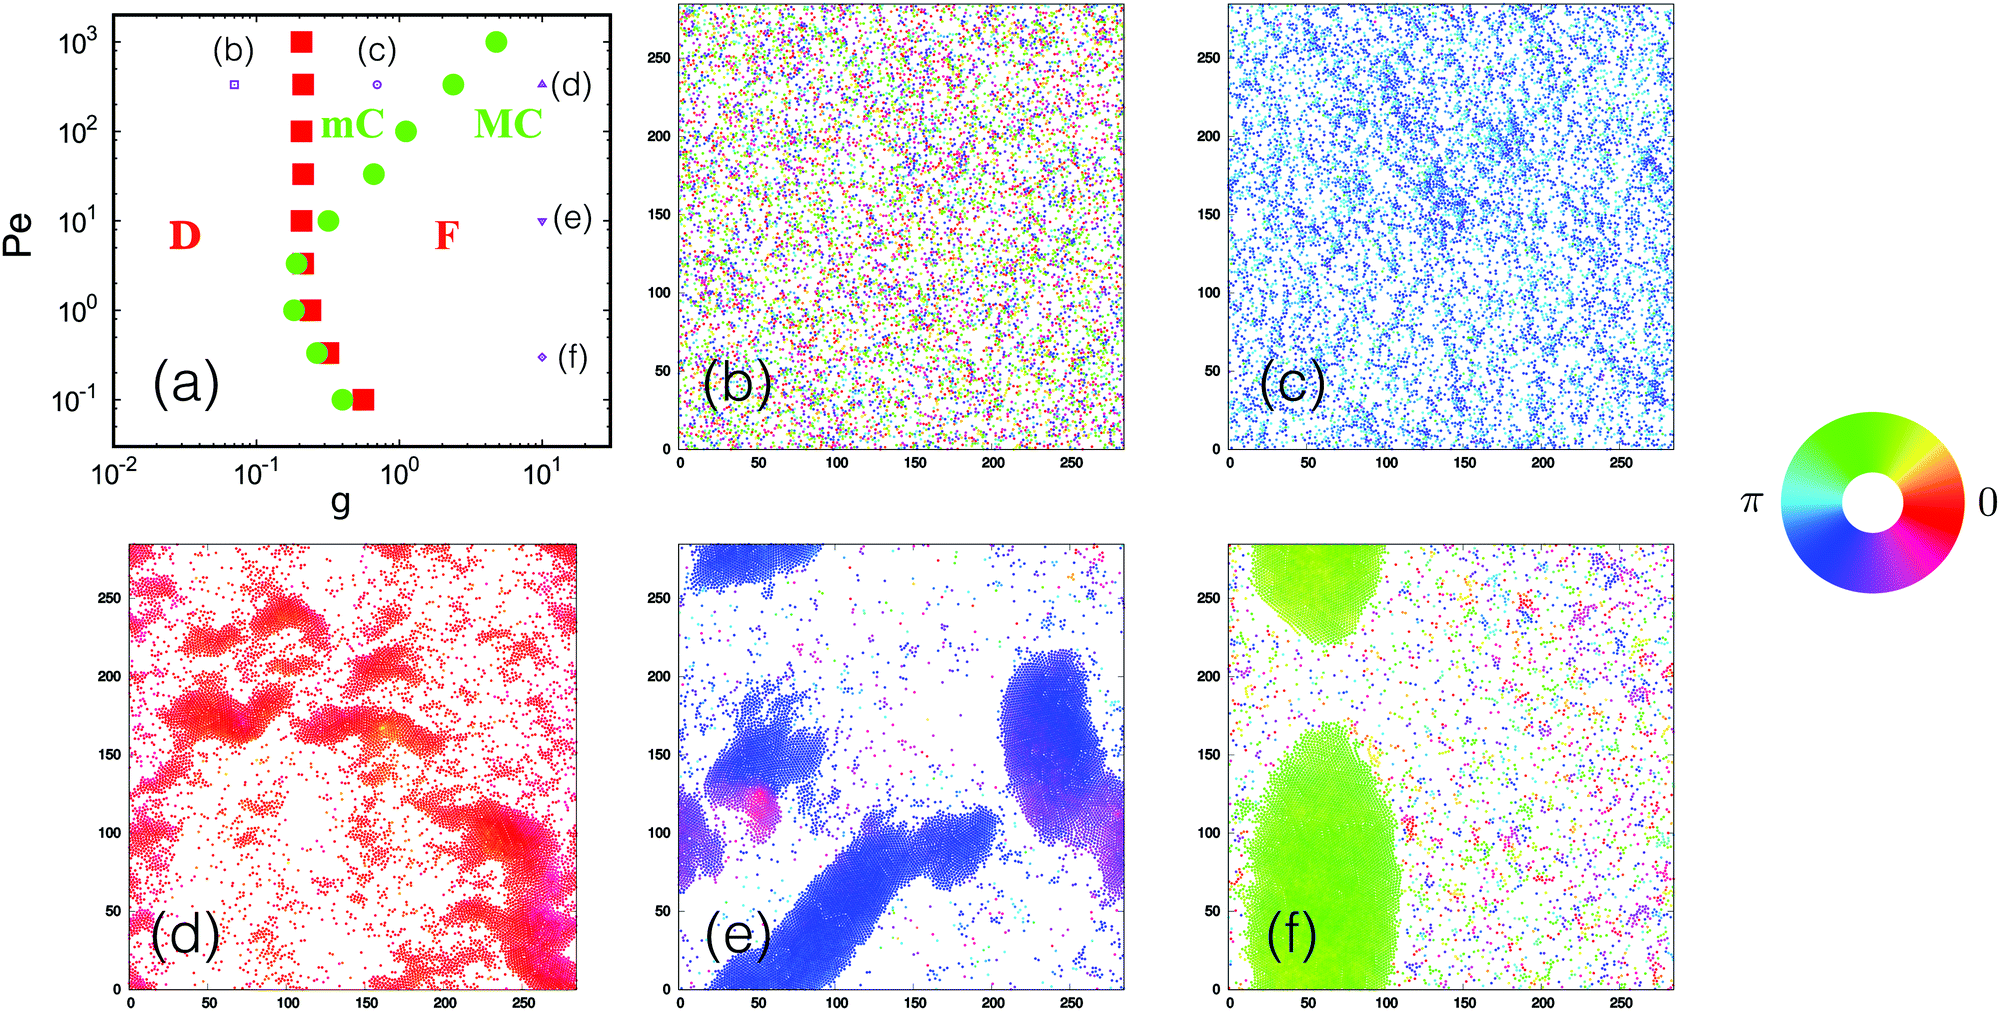
\includegraphics[width=\textwidth]{martin_phaseseparation.png}
			\label{fig:martin_flocking1}
			\caption{\cite{martin-gomez_collective_2018}}
		\end{figure}
		
		After noting that the phase transition happens with increasing $g$ for any $\mathrm{Pe} > 1$, authors focus on studying this transition in $g$, in the  spirit of an equilibrium phase transition, with $P$ as the order parameter and its susceptibility $\chi = N(\langle P^2 \rangle - \langle P \rangle^2)$. The behavior of the two quantities is similar to what is expected in a continuous phase transition with the critical coupling $g^c = 0.21 \pm 0.02$ (Figure \ref{fig:martin_flocking3}(a)).
		
		In the next part authors focus on clustering phenomena, noting that the cluster size distribution decays exponentially for $g < g*$ and algebraically for $g > g*$. This defines the two phases of microscopic and macroscopic clustering.
		Introducing two new order parameters
		\[ P_x = \left\langle \left| \frac{1}{N} \sum_{i=1}^N \cos(\theta_i) \right| \right\rangle ; \quad
		P_y = \left\langle \left| \frac{1}{N} \sum_{i=1}^N \sin(\theta_i) \right| \right\rangle,
		 \]
		 it is possible to distinguish between lane-like and band-like behavior in aligned clusters.
		 
		 \begin{figure}[htp]
		 	\centering
		 	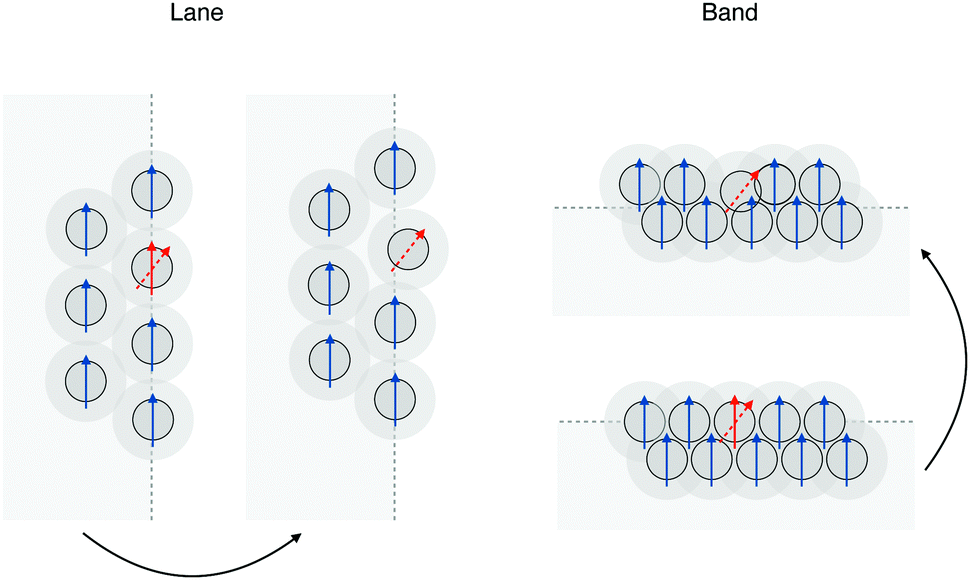
\includegraphics[width=.7\textwidth]{martin_laneband.png}
		 	\label{fig:martin_flocking2}
		 	\caption{\cite{martin-gomez_collective_2018}}
		 \end{figure}
		 
		 The authors use the radial distribution function 
		 \[ g(r) = \frac{1}{N} \left\langle \sum_{j \neq i} \sum_{i} \delta \left( r - |\mathbf{r}_i - \mathbf{r}_j| \right) \right\rangle
		  \]
		to characterize the global structure of the largest cluster. Increasing the coupling $g$ at fixed Péclet number makes the peaks higher and shifts them to larger distances, showing that the system is developing a longer range order.
		
		\begin{figure}[htp]
			\centering
			\subfloat[][Polarization and its susceptibility]{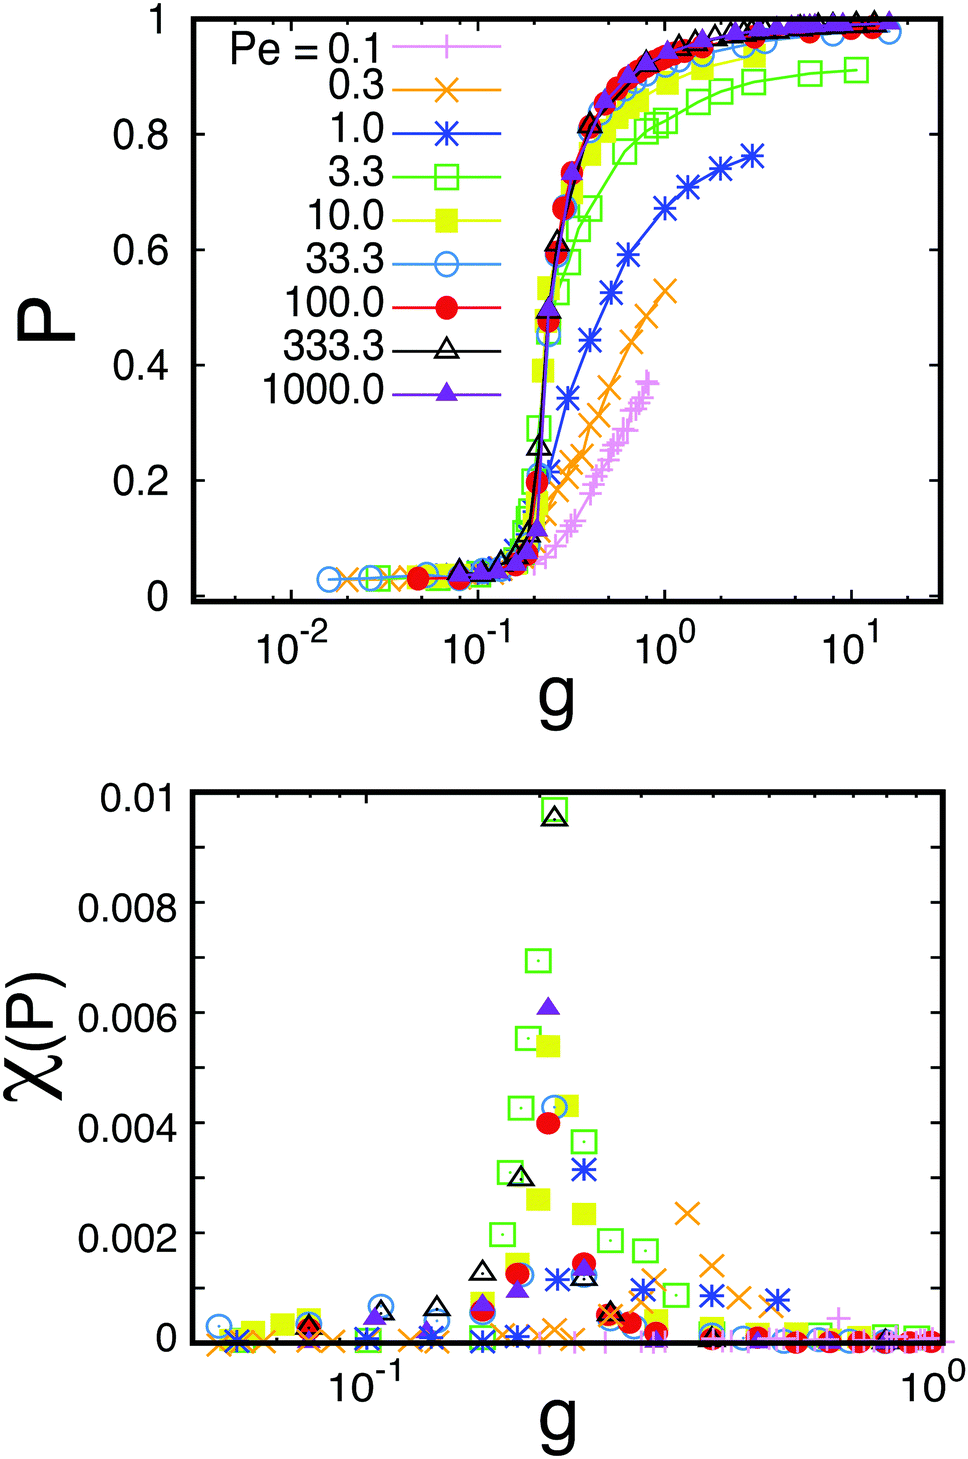
\includegraphics[width=0.45\textwidth]{martin_phasetransition.png}}\quad
		    \subfloat[][Pair correlation function and static structure factor]{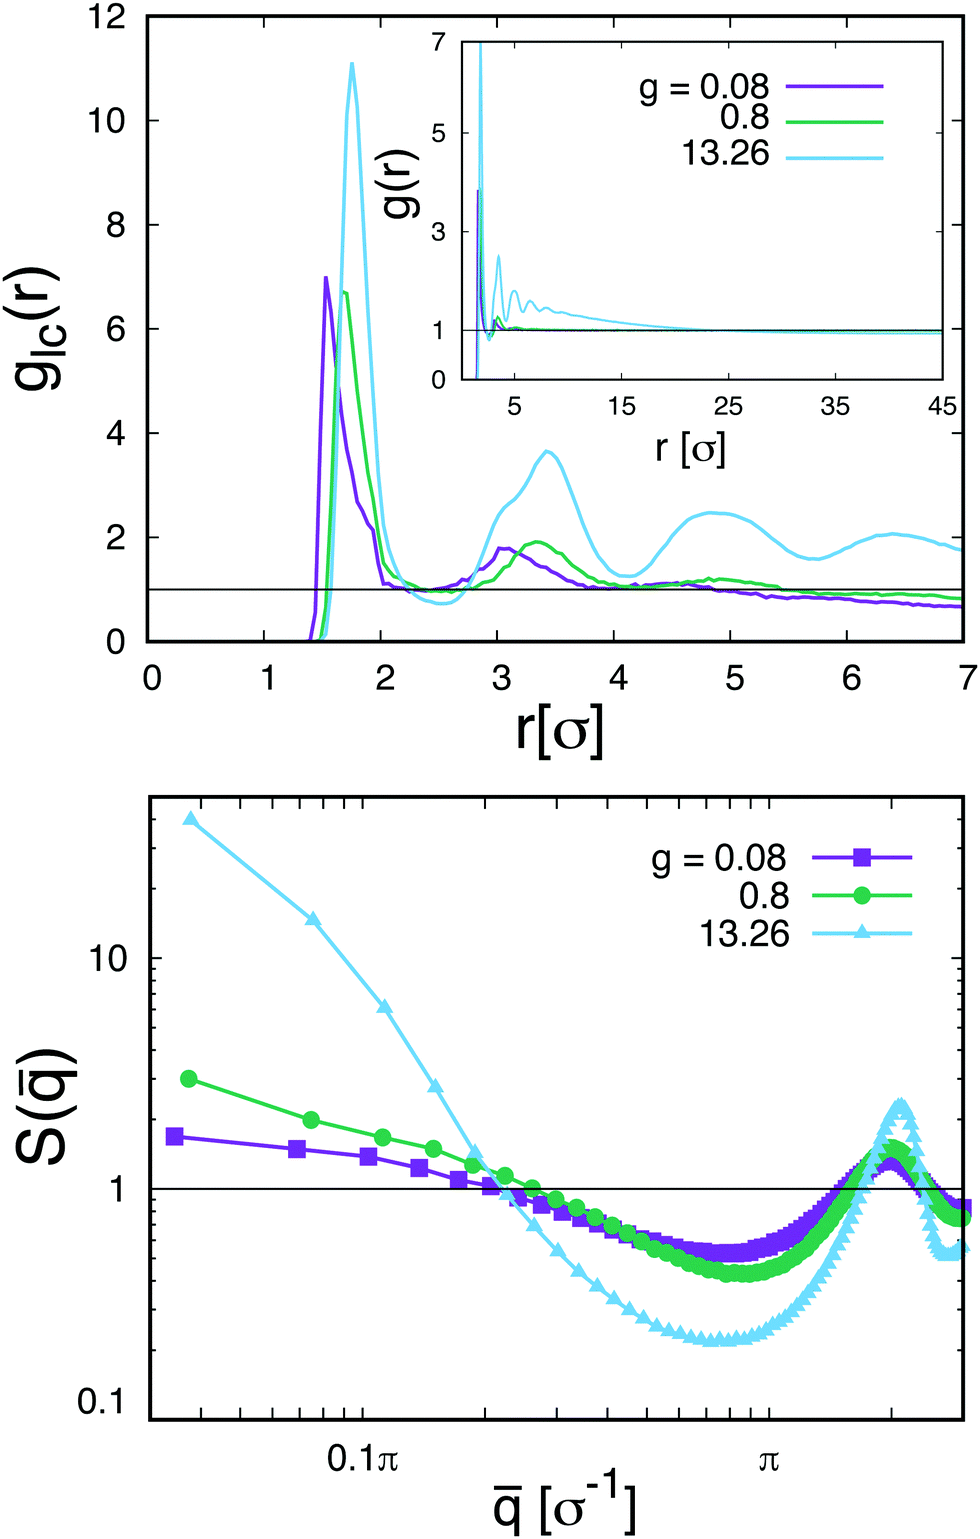
\includegraphics[width=0.45\textwidth]{martin_gofr.png}}
		    
		    \caption{\cite{martin-gomez_collective_2018}}
		    \label{fig:martin_flocking3}
		\end{figure}
		
		In \cite{caprini_spontaneous_2020}, authors investigate the alignment of instantaneous velocities in cases where motility-induced phase separation occurs. Most literature focuses on the effect that a central 2-body potential, or an explicit aligning interaction which couples the orientational degrees of freedom of single particles, has on the system, but the interplay between phase separation of particles systems and alignment in their velocity has hardly been studied.
		
		In the aforementioned paper, it is shown how, when ABPs systems with a simple repulsive only Weeks-Chandler-Anderson potential phase-separate in a cluster, their velocity tend to form aligned domains, regardless the self propulsion orientation. For this reason, the global polarization is not a good order parameter, even when the computation is restricted to clusters, thus the authors introduce the spatial correlation function of the velocity orientation $Q_i(r) = 1-2\sum_{j} \frac{d{ij}}{\mathcal{N}_k \pi } $, being $d_{ij} = \mathrm{min}\left[|\theta_i - \theta_j|, 2 \pi - |\theta_i - \theta_j| \right]$ the angular distance between two particles and $\mathcal{N}_k$ is the number of particles in a circular shell around the i-th particle, taken with a thickness $\bar{r} = \mathrm{argmax} \{g(r)\}$, and mean radius $k\bar{r}$ with integer $k$. 
		
		It is possible to derive an order parameter from $Q(R)$ integrating it
		\[ 
		R = \int Q(r) dr \]
		where the integral is performed on the cluster domain when present. 
		This seems to be a good order parameter: varying the reorientation time $1/D_r$, $R$ is discontinuous at the point where the MIPS occurs and the result is consistent with established MIPS order parameters as shown in Figure \ref{fig:caprini1}.
		
		\begin{figure}[htp]
			\centering
			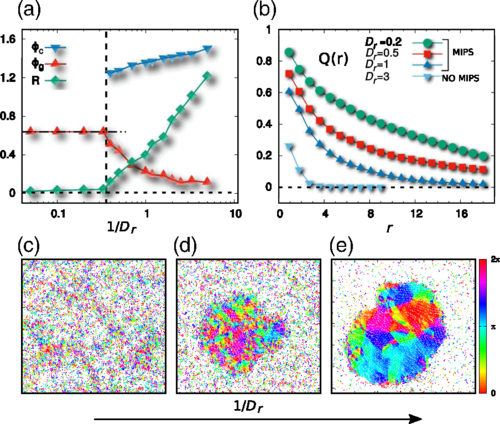
\includegraphics[width=\textwidth]{caprini2.png}
			\label{fig:caprini1}
			\caption{\cite{caprini_spontaneous_2020}}
		\end{figure}
		
		Going on, the article shows analitically how it is possible to rewrite the equation of motion for the velocity: considering the symmetry in the hexagonal lattice which the particles arrange into, such equation involves a term which depends on the difference between particle's velocity and average velocity of the six surrounding it, thus re-obtaining a Vicsek-like model without a specific aligning interaction.
\end{document}